\chapter{Spettroscopia}

Un pilastro informativo in astrofisica è l'analisi dei profili spettrali, noto come \textbf{sprettroscopia}, in grado di dare molte informazioni riguardo le sorgenti, in quanto ogni profilo è tipico di un certo tipo di processo di emissione ed è quindi utile per capire la fisica che sta dietro i segnali che riceviamo. L'incipit di questa analisi sta innanzitutto in un processo di isolamento e collimazione della luce proveniente dalla specifica sorgente che si vuole studiare, tipicamente svolto dal telescopio, dopo di che il fascio viene fatto espandere tramite una fenditura, posta solitamente nel fuoco stesso del telescopio, per poi passare attraverso un \textit{elemento dispersivo}, come ad esempio un prisma. L'elemento dispersore rende possibile l'analisi dello spettro spacchettando il fascio in arrivo in tutte le lunghezze d'onda, per rendere questo possibile è necessario che il fascio incidente arrivi parallelo, poichè la rifrazione è in funzione sia della lunghezza che dell'angolo incidente.

\begin{figure}[h]
    \centering
    \vspace{-5pt}
    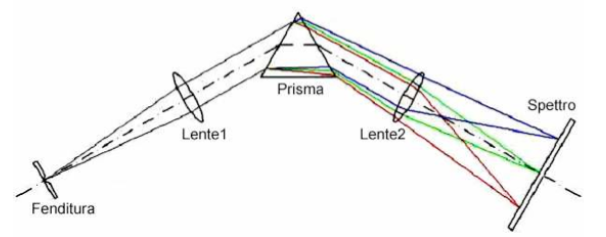
\includegraphics[width=0.5\textwidth]{Immagini/Capitolo3/Spettroscopia_schema.PNG}
    \caption*{Rappresentazione schematica di uno spettroscopio a prisma}
    \vspace{-5pt}
\end{figure}

Per togliere quest'ultimo elemento e analizzare solo il percorso di rifrazione, si introducono delle lenti focalizzanti tra la fenditura e il prisma, ma anche tra il prisma e successivamente il piano focale, per cui il fascio incida da prima parallelamente, per poi essere reso ancora più separato a seguito della dispersione sul piano focale, in modo da rendere l'analisi più effettiva. I fasci uscenti, separati ulterioramente dal secondo specchio, andranno poi fuocheggiati da un secondo obiettivo, per fare ciò si regola il sistema ottico in modo da inviare lo spettro orientato lungo uno degli assi del CCD.

\begin{wrapfigure}{l}{0.35\textwidth}
    \centering
    \vspace{-5pt}
    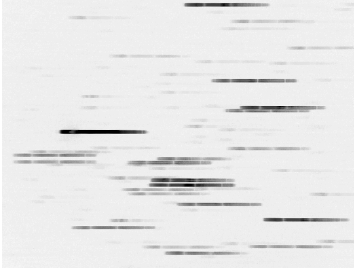
\includegraphics[width=0.34\textwidth]{Immagini/Capitolo3/Spettro_cielo_generico.PNG}
    \caption*{Spettro generico di una parte di cielo, direzione di dispersione orizzontale verso destra}
    \vspace{-5pt}
\end{wrapfigure}

Questa tecnica a prisma crea un'immagine a righe, le quali si estendono tutte in una direzione specifica, che è la \textit{direzione di dispersione}, come si vede in immagine, la quale è frutto di uno spettroscopio in cui si è osservato un pezzo di cielo, senza isolare una sorgente specifica, per cui ad ogni riga corrisponde una differente sorgente. Per passare ad una descrizione più formale, risulta necessario partire proprio dal concetto di \textit{dispersione angolare} $d\beta/d\lambda$, che consiste, come è facilmente intuibile, nella differenza di angolo di dispersione $d\beta$ rapportato alla differenza di lunghezza d'onda $d\lambda$ tra due onde adiacenti. A seguito della dispersione, le onde vengono poi focalizzate su un CCD, che una volta calibrato avrà la sua focale equivalente $f$. Ora, se i raggi arrivano paralleli opichè rifocalizzati, significa che ad ogni raggio disperso ad angolo $\beta$ corrisponderà una distanza diversa sul piano focale, chiamando $l$ la distanza dall'asse ottico e ricordando la correlazione diretta tra angolo di dispersione e distanza lineare sul piano focale, si ricava la dispersione lineare:
\begin{equation}
    \frac{dl}{d\lambda} = f \frac{d\beta}{d\lambda}
\end{equation}
Dove la dispersione angolare è quella propria dell'elemento dispersore dell'apparato. La misura finale dello shift lineare può essere sia in $mm/\angstrom$ che più comodamente in $pxl/\angstrom$, essendo i pixel quello con cui poi si va effettivamente a lavorare, un esempio della comodità di avere un'equazione espressa nelle seconde è avere un riferimento diretto a quanti pixel di differenza ci siano per una variazione $d\lambda$ di lunghezza d'onda.

\begin{wrapfigure}{r}{0.4\textwidth}
    \centering
    \vspace{-10pt}
    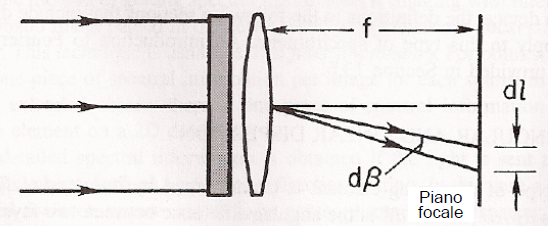
\includegraphics[width=0.39\textwidth]{Immagini/Capitolo3/Spettroscopia_schema_dispersione_lineare.PNG}
    \caption*{Schema dispersione lineare}
    \vspace{-10pt}
\end{wrapfigure}

Questa quantità viene spesso usata nel suo inverso, per motivi di pura comodità, ossia come $d\lambda/dl$, ovviamente con le unità invertite che siano $\angstrom/mm$ o $\angstrom/pxl$, in tal senso viene inteso come campionamento in pixel lungo la direzione di dispersione delle onde al variare della propria lunghezza d'onda. Così come è importante, nel caso visto di imaging, non confondere la risoluzione angolare di un sistema ottico con il suo campionamento, allo stesso modo in spettroscopia non va confusa la dispersione lineare di uno spettrografo con la sua risoluzione. Parlando di ciò, si definisce la \textbf{risoluzione spettrale} $R$ di uno spettrografo come la capacità di risolvere onde a lunghezza d'onda vicine, formalmente si definisce come:
\begin{equation}
    \label{def:risoluzione-spettrale}
    R = \frac{\lambda}{\Delta\lambda}
\end{equation}